%%%%%%%%%%%%%%%%%%%%%%%%%%%%%%%%%%%%%%%%%%%%%%%%%%%%%%%%%%%%%%%%%%%%
%% I, the copyright holder of this work, release this work into the
%% public domain. This applies worldwide. In some countries this may
%% not be legally possible; if so: I grant anyone the right to use
%% this work for any purpose, without any conditions, unless such
%% conditions are required by law.
%%%%%%%%%%%%%%%%%%%%%%%%%%%%%%%%%%%%%%%%%%%%%%%%%%%%%%%%%%%%%%%%%%%%

\documentclass{beamer}
\usetheme[faculty=phil]{fibeamer}
\usepackage[utf8]{inputenc}
\usepackage[
  main=english
]{babel}
%% These macros specify information about the presentation
\title{Classical Black Holes} %% that will be typeset on the
\subtitle{06. Astrophysics of Supermassive Black Holes} %% title page.
\author{Edward Larra\~{n}aga}
%% These additional packages are used within the document:
\usepackage{ragged2e}  % `\justifying` text
\usepackage{booktabs}  % Tables
\usepackage{tabularx}
\usepackage{tikz}      % Diagrams
\usetikzlibrary{calc, shapes, backgrounds}
\usepackage{amsmath, amssymb}
\usepackage{url}       % `\url`s
\usepackage{listings}  % Code listings
\usepackage{siunitx}
\frenchspacing
\begin{document}
\frame{\maketitle}

\AtBeginSection[]{% Print an outline at the beginning of sections
\begin{frame}<beamer>
\frametitle{Outline for Part \thesection}
\tableofcontents[currentsection]
\end{frame}}

\section{Supermassive Black Holes in the Astrophysical Scenario}

\subsection{Supermassive Black Holes}
\begin{frame}{Supermassive Black Holes}
	Astrophysical observations have discovered evidence of the existence of black holes, with masses in the range $M \sim 10^5 - 10^{10} M_\odot\ $.\\
	\bigskip
	\pause

	Dynamical evidence supports that supermassive black holes are located at the center of almost all galaxies (there are some exceptions such as the galaxy A2261-BCG).
	\bigskip
	\pause
	
	In the Milky Way, the central black hole, called Sagittarius A* has a mass $\sim 4 \times 10^6 M_\odot\ $.
\end{frame}

\subsection{Origin of Supermassive Black Holes}
\begin{frame}{Origin of Supermassive Black Holes}
	There are many hypotheses on the origin of supermassive black holes. For example:
	\begin{itemize}
    \item<2-> Gravitational collapse of the first generation of stars (Population III).
    \item<3-> Gas-dynamical instabilities.
	\item<4-> Stellar-dynamical stabilities.
	\item<5-> Dark Matter collapse
	\item<6-> Primordial fluctuations
    \end{itemize}
\end{frame}

\begin{frame}{Origin of Supermassive Black Holes}
	The first hypothesis on the origin of supermassive black holes states that,\\
	\bigskip
	\onslide<1-> Population III stars are formed out of the collapse of zero-metallicity gas.\\
	\pause
	\bigskip
	\onslide<2-> These stars are expected to be very massive, $M_* > 100 M_\odot\ $\\
	\pause
	\bigskip
	\onslide<3-> Then, they will die with a gravitational collapse, leaving behind black holes with masses between $40$ and $1000 M_\odot\ $ \\
	\pause
	\bigskip
	\onslide<4-> After that, Galaxies formed around these early black holes.
\end{frame}

\begin{frame}{Origin of Supermassive Black Holes}
	The mechanism of gas-dynamical instabilities states that\\
	\pause
	\bigskip
	\onslide<2-> If fragmentation is inhibited in early massive cloud by, for example, turbulences, and cooling proceeds gradually, the gas will contract until rotation stops the collapse.\\ 
	\pause
	\bigskip
	\onslide<3-> Then, global dynamical instabilities (like bar-instabilities) can transport angular momentum outwards, allowing the core collapse to continue.\\ 
	\pause
	\bigskip
	\onslide<4-> The gas accumulated in the center producea very massive central object producing a black hole with a mass of $ \sim 10^4 M_\odot\ $ or higher.
\end{frame}

\begin{frame}{Origin of Supermassive Black Holes}
	The mechanism of stellar-dynamical stabilities states that\\
	\pause
	\bigskip
	\onslide<2-> If fragmentation occurs, star formation in a collapsing cloud of gas produces a compact nuclear stellar cluster.\\ 
	\pause
	\bigskip
	\onslide<3-> Collisions of stars in the cluster are frequent and they can produce a black hole of $ \sim 10^2 - 10^4 M_\odot\ $ \\ 
\end{frame}

\begin{frame}{Origin of Supermassive Black Holes}
	The mechanism of Dark Matter collapse states that\\
	\pause
	\bigskip
	\onslide<2-> Dark matter collapse proceeds as described for a cloud of dust.\\ 
	\pause
	\bigskip
	\onslide<3-> No heating in the collapse until the rate of annihilation of dark particles becomes significant.\\ 
	\pause
	\bigskip
	\onslide<4-> This process create an object called a \textit{Dark Matter Star} for which the annihilation radiation supports the gravitational collapse.
\end{frame}

\begin{frame}{Origin of Supermassive Black Holes}
	\onslide<1-> The temperature of this Dark Matter star is estimated between $4000$ and $10000$ \si{K} and its radius of approximately $10^{12}$ \si{m}.\\
	\pause
	\bigskip
	\onslide<2-> The luminosity of these objects is about $10^6 L_\odot\ $ and their mass is estimated in $1000 M_\odot\ $\\ 
	\pause
	\bigskip
	\onslide<3-> When the dark matter is completely annihilated, the object will collapse into a massive black hole.
\end{frame}

\begin{frame}{Origin of Supermassive Black Holes}
	\onslide<1-> The last hypothesis for the origin of supermassive black holes is from primordial fluctuations.\\
	\pause
	\bigskip
	\onslide<2-> At the regions where the density fluctuations are large enough, the gravitational force may overcome the pressure, giving as a result a complete collapse.\\ 
	\pause
	\bigskip
	\onslide<3-> This process create primordial black holes with masses up to $\sim 1000 M_\odot\ $. \\
\end{frame}


\subsection{Intermediate Black Holes}
\begin{frame}{Physical Aspects of the Stellar Death}
	\onslide<1-> 
    Nuclear reactions $\rightarrow$ thermal pressure $\rightarrow$ support gravity \\
    \bigskip
    \onslide<2-> 
    For massive stars $(M > 5M_\odot\ )$,\\
    H $\rightarrow$ He $\rightarrow$ ... $\rightarrow$ C $\rightarrow$ ... $\rightarrow$ Fe
\end{frame}

\begin{frame}{White Dwarf. Degenerate Gas of Electrons}
	\onslide<1-> Equation of State for the degenerate gas of electrons
    \onslide<2-> 
    $$P_{rel} = K \rho^{4/3}$$
    \onslide<3-> Using $\frac{dP(r)}{dr} = -\frac{GM(r)\rho(r)}{r^2}$ we obtain 
    \onslide<4-> 
    $$\frac{M^{4/3}}{r^5} \propto \frac{GM^2}{r^5} $$
\end{frame}

\begin{frame}{Chandrasekhar's Limit (1931)}
	\onslide<1-> 
    $$\frac{M^{4/3}}{r^5} \propto \frac{GM^2}{r^5} $$
    \onslide<2-> This relations is satisfied by the unique mass
    $$M_C = 0.197 \left[ 
    	\left( \frac{hc}{G}\right)^3 \frac{1}{m_p^2} \right] \frac{1}{\mu^2_e}$$
    \onslide<3-> $\mu_e$: mean molecular wight of the electrons
	\onslide<4-> 
	$$M_C \approx 1.4 M_\odot\ $$
    Mass of a completely degenerated star.
\end{frame}

\begin{frame}{Neutron Stars. Degenerate Gas of Neutrons}
	\onslide<1-> Chandrasekhar (1939)\\
    \onslide<2-> If the degenerate star attains sufficiently high densities, the protons and electrons will combine to form neutrons.\\
    \bigskip
    \onslide<3-> Baade and Zwicky (1934)\\
	\onslide<4-> "...supernovae represent the transitions from ordinary stars into neutron stars which in their final stages consist of extremely closely packed neutrons."\\
\end{frame}
        
\begin{frame}{Neutron Stars. Degenerate Gas of Neutrons}
	\onslide<1-> 
    Oppenheimer and Volkoff (1939)\\
    Oppenheimer and Snyder (1939)\\
    \onslide<2-> \justify{“...when all thermonuclear sources of energy are exhausted a sufficiently heavy star will collapse. This contraction will continue indefinitely till the radius of the star approaches asymptotically its gravitational radius. Light from the surface of the star will be progressively reddened and can escape over a progressively narrower range of angles till eventually the star tends to close itself off from any communication with a distant observer”.}
\end{frame}

\begin{frame}{Black Holes}
	If the collapsing core is too massive to be supported by the degenerate pressure of neutrons, there is no known mechanism capable of finding a new equilibrium configuration, and the body should undergo a complete collapse.
    \bigskip
    
    In this case, the final product is a black hole.
\end{frame}

\section{Mathematical Description of the Collapse}    
\begin{darkframes}

\subsection{Spherically Symmetric Collapse}
\begin{frame}{Spherically Symmetric Collapse}
	\begin{itemize}
	\item<1-> Spherical Symmetry:
    $$ds^2 = -e^{2\alpha(t,r)}dt^2 + e^{2\beta(t,r)}dr^2 + R^2(t,r) d\Omega^2$$  
	\item<2-> Suppose that the collapsing body can be described as a perfect fluid. \\
    Then, we consider that coordinates $t$ and $r$ are attached to every collapsing particle (co-moving coordinates).
    \end{itemize}
\end{frame}

\begin{frame}{Spherically Symmetric Collapse}
	\begin{itemize}
	\item<1-> In the co-moving frame, the 4-velocity of the fluid is just
    $$ u^\mu = \left( e^{-\alpha},0,0,0 \right)$$
    and thus $u^2 = -1$.
    \item<2-> The energy-momentum tensor in the co-moving frame is
    $$T^\mu_\nu = diag(\rho, P,P,P)$$
    \end{itemize}
\end{frame}

\begin{frame}{Spherically Symmetric Collapse}
	The Einstein equations for this metric give
	$$
    \begin{array}{c c c}
    G^t_t = 8\pi T^t_t &\Rightarrow &\frac{F'}{R^2 R'} = 8\pi \rho \\
    G^r_r = 8\pi T^r_r &\Rightarrow &\frac{\dot{F}}{R^2 \dot{R}} = -8\pi P \\
   	G^t_r = 0 &\Rightarrow & \dot{R}'-\dot{R} \alpha'-\dot{\beta} R' =0 \\
    \end{array}$$
    \pause
    $$F = R \left( 1 - e^{-2\beta} R'^2 + e^{-2\alpha} \dot{R}^2  \right)$$
    \centering
    Misner-Sharp mass
\end{frame}

\begin{frame}{Spherically Symmetric Collapse}
	The Misner-Sharp mass
    $$F = R \left( 1 - e^{-2\beta} R'^2 + e^{-2\alpha} \dot{R}^2  \right)$$
    is defined by the relation
    $$1 - \frac{F}{R} = g_{\mu\nu} \left( \partial^\mu R \right) \left( \partial^\nu R \right)$$
    \pause
    \footnotesize
    * Note that $n^\mu = \partial^\mu R$ is normal to the surfaces $R = \textrm{constant}$.\\ 
    Thus, when $1 - \frac{F}{R} = 0$, the corresponding surface is null.
\end{frame}

\begin{frame}{Spherically Symmetric Collapse}
	From $(t,t)$-component of the Field equations we obtain the Misner-Sharp mass as
    $$G^t_t = 8\pi T^t_t \Rightarrow \frac{F'}{R^2 R'} = 8\pi \rho$$
    \pause
    $$ F(r) = \int_0^r F' d\tilde{r} = 8\pi \int_0^r \rho R^2 R' d\tilde{r} = 2M(r) $$
\end{frame}
     
\begin{frame}{Spherically Symmetric Collapse}
	Finally, the conservation of the energy-momentum tensor gives the equation
    $$\nabla_\mu T^\mu _\nu = 0 \Rightarrow \alpha'= - \frac{P'}{\rho + P}$$
\end{frame}

\subsection{Dust Collapse}
\begin{frame}
	\huge
	Dust Collapse
\end{frame}

\begin{frame}{Dust Collapse}
	Dust is characterized by $P=0$.
    \pause
	$$
    \begin{array}{c c c}
    G^t_t = 8\pi T^t_t &\Rightarrow &\frac{F'}{R^2 R'} = 8\pi \rho \\
    G^r_r = 8\pi T^r_r &\Rightarrow &\frac{\dot{F}}{R^2 \dot{R}} = 0 \\
   	G^t_r = 0 &\Rightarrow & \dot{R}'-\dot{R} \alpha'-\dot{\beta} R' =0 \\
    \nabla_\mu T^\mu _\nu = 0 &\Rightarrow &\alpha'= 0
    \end{array}
    $$
    \pause
    Then
    \begin{align*}
    F &= F(r)\\
    \alpha &= \alpha(t)
    \end{align*}
\end{frame}

\begin{frame}{Dust Collapse}
	$F = F(r)$: No inflow or outflow of energy through spherical shells. Thus, the exterior metric is Schwarzschild.
    \bigskip
    
    \pause
    If the boundary of the cloud of dust is located at the co-moving coordinate $r=r_b$, we have $F(r_b) = 2M$ with $M$ the Schwarzschild's mass of the exterior metric.
    \bigskip
    
    \pause
    \footnotesize
    * If $P\neq0$ the exterior metric must be a non-vacuum Vaidya spacetime.
\end{frame}

\begin{frame}{Dust Collapse}
    $\alpha = \alpha(t)$: One can re-define the time coordinate such that
    $$  e^{\alpha(t)} dt \Rightarrow dt$$
    and therefore $g_{tt} = -1$
\end{frame}

\begin{frame}{Dust Collapse}
    $$\dot{R}'-\dot{R} \alpha'-\dot{\beta} R' = 0$$
    \pause
    $$\dot{R}'-\dot{\beta} R' =0$$
    \pause
    $$\frac{1}{R'} \frac{d(R')}{dt} = \frac{d\beta}{dt}$$
    \pause
    $$\frac{d(\log R')}{dt} = \frac{d\beta}{dt}$$
    \pause
    $$R' = e^{\beta + h(r)}$$
\end{frame}

\begin{frame}{Dust Collapse}
    $$R' = e^{\beta + h(r)}$$
    \pause
    Introducing $f(r) = e^{2h(r)} - 1$ we have
    $$ e^{2\beta} = \frac{R'^2}{1+f}$$
\end{frame}

\begin{frame}{Dust Collapse}
    $$ds^2 = -dt^2 + \frac{R'^2(t,r)}{1+f(r)} dr^2 + R^2(t,r) d\Omega^2 $$
    \centering
    Lemaitre-Tolman-Bondi Metric
\end{frame}

\begin{frame}{Dust Collapse}
    Kretschmann Scalar:
    $$K = 12\frac{F'^2}{R^4 R'^2} - 32\frac{FF'}{R^5 R'} + 48 \frac{F^2}{R^6}$$
    \pause
    Divergence at $R=0$
\end{frame}

\begin{frame}{Dust Collapse}
    One can re-scale to set $R(t,r)$ to equal the co-moving radius $r$ at the time $t=0$, i.e. we impose $R(0,r)=r$ and introduce a scale factor $a$ such that
    $$R(t,r) = r a(t,r)$$

	$a(0,r) = 1$\\
    \pause
    
    $a(t_s,r) = 0$ (at the time of the formation of the singularity, $t=t_s$)\\
    \bigskip
    \pause
    The collapse also impose the condition $\dot{a}<0$ 
\end{frame}

\begin{frame}{Dust Collapse}
    One of the field equations,
    $$\frac{F'}{R^2 R'} = 8\pi \rho$$
    implies that a regular value of the density at $t=0$ is obtained if the Misner-Sharp mass has the form
    $$F(r) = r^3 m(r)$$
    where $m(r)$ is a (sufficiently) regular function in the region $[0,r_b]$.
\end{frame}

\begin{frame}{Dust Collapse}
    We have $F' = 3r^2 m + r^3 m'$ and therefore
    $$\frac{F'}{R^2 R'} = 8\pi \rho$$
    \pause
    $$\frac{3r^2 m + r^3 m'}{(ra)^2 (a+ra')} = 8\pi \rho$$
    \pause
    $$\frac{3m + r m'}{a^2 (a+ra')} = 8\pi \rho$$
\end{frame}

\begin{frame}{Dust Collapse}
    It is usual to consider $m(r)$ as a polynomial around $r=0$,
    $$m(r) = \sum_{k=0} ^\infty m_k r^k$$
    where $m_k$ are constants
\end{frame}

\begin{frame}{Dust Collapse}
    From the definition of the Misner-Sharp mass we have
    $$\dot{R}^2 = \frac{F}{R} + f$$
    \pause
    Using the proposed forms for $F$ and $R$ we obtain
    $$r \dot{a} = - \sqrt[]{\frac{mr^2}{ra}+f}$$
    \pause
    $$\dot{a} = - \sqrt[]{\frac{m}{a}+\frac{f}{r^2}}$$
\end{frame}

\begin{frame}{Dust Collapse}
    Evaluating at the time $t=0$ we have $a(0,r)=1$ and thus
    $$\dot{a}(0,r) = - \sqrt[]{m+\frac{f}{r^2}}$$
    \pause
    Note that the function $f$ defines the initial velocity of the particles in the cloud.
    \pause
    It is usual to write this function as an expansion around $r=0$ as
    $$f(r) = r^2 b(r)$$
    with
    $$ b(r) = \sum_{k=0}^\infty b_k r^k$$
\end{frame}

\subsection{Homogeneous Dust Collapse}
\begin{frame}
	\huge
    {Homogeneous Dust Collapse}
\end{frame}

\begin{frame}{Homogeneous Dust Collapse}
    Simplest Model of Gravitational Collapse. Oppenheimer-Snyder (1939)\\
    \bigskip 
    
    \pause
    Homogeneous: $\rho = \rho (t)$\\
    \pause
    \bigskip
    
    This implies that \\
    $m'=0 \longrightarrow  m = m_0$\\
\end{frame}

\begin{frame}{Homogeneous Dust Collapse}
    Simplest Model of Gravitational Collapse. Oppenheimer-Snyder (1939)\\
    \bigskip
    
    \pause
    It also implies that\\
    \bigskip
    
    $a'=0 \longrightarrow \frac{f}{r^2}=\textrm{constant}$\\ 
    \pause
    $f(r) = r^2 b(r) = r^2 \textrm{constant}$\\
    \pause
    which is accomplished by choosing $b=b_0$\\
    \pause
  	Then
    $$ \dot{a} = -\sqrt[]{\frac{m_0}{a}+b_0}$$
\end{frame}

\begin{frame}{Homogeneous Dust Collapse}
    The Lemaitre-Tolman-Bondi line element becomes
 	$$ds^2 = -dt^2 + \frac{R'^2(t,r)}{1+f(r)} dr^2 + R^2(t,r) d\Omega^2 $$
    \pause
  	$$ds^2 = -dt^2 + \frac{a^2(t)}{1+r^2 b_0} dr^2 + r^2 a^2(t) d\Omega^2 $$
    \pause
   	$$ds^2 = -dt^2 + a^2(t) \left[ \frac{dr^2}{1+b_0 r^2} + r^2 d\Omega^2 \right] $$
\end{frame}

\begin{frame}{Homogeneous Dust Collapse}
   	$$ds^2 = -dt^2 + a^2(t) \left[ \frac{dr^2}{1+b_0 r^2} + r^2 d\Omega^2 \right] $$
    For $b_0=0$ this line element becomes
    $$ds^2 = -dt^2 + a^2(t) \left[ dr^2 + r^2 d\Omega^2 \right] $$
    and describes the counterpart of a flat spacetime, in which the collapse is marginally bound (i.e. the falling particles have vanishing velocity at infinity).
\end{frame}

\begin{frame}{Homogeneous Dust Collapse}
   	For $b_0 =0$ the scale factor is
    $$ \dot{a} = -\sqrt[]{\frac{m_0}{a}+b_0}$$
    \pause
    $$ \frac{da}{dt} = -\sqrt[]{\frac{m_0}{a}}$$
    \pause
    $$ \sqrt[]{a} da = -\sqrt[]{m_0} dt$$
    \pause
    $$ \frac{2}{3} a^{3/2} - \frac{2}{3} a^{3/2}(0) = -\sqrt[]{m_0} t$$
\end{frame}

\begin{frame}{Homogeneous Dust Collapse}
    The value of the initial condition was supposed as $a(0)=1$. Thus
    $$a(t) = \left[ 1-\frac{3\sqrt[]{m_0}}{2}t \right]^{2/3}$$
    \pause
    Therefore, the singularity $ R=0 $ occurs at the time $t_s$ for which $a(t_s)=0$. This is
    $$t_s = \frac{2}{3\sqrt[]{m_0}}$$
\end{frame}

\begin{frame}{Homogeneous Dust Collapse}
    The curve $t_H (r)$ describing the time at which the shell $r$ crosses the  horizon can be obtained from the condition
    $$1-\frac{F}{R} = 0$$
    \pause
    $$1-\frac{m_0 r^3}{r a(t_H)} = 0$$
    \pause
    $$a(t_H)=m_0 r^2$$
\end{frame}

\begin{frame}{Homogeneous Dust Collapse}
    $$a(t_H)=m_0 r^2$$
    \pause
    For $b_0 = 0$ wehave
    $$ \left[ 1-\frac{3\sqrt[]{m_0}}{2}t_H \right]^{2/3} = m_0 r^2$$
    \pause
    $$t_H (r) = \frac{2}{3\sqrt[]{m_0}} - \frac{2}{3} m_0 r^3$$
\end{frame}

\end{darkframes}
\begin{frame}{Gravitational Collapse of a Homogeneous Cloud of Dust}
\framesubtitle{Eddington-Finkelstein Diagram}
	\begin{center}
      \begin{figure}
      	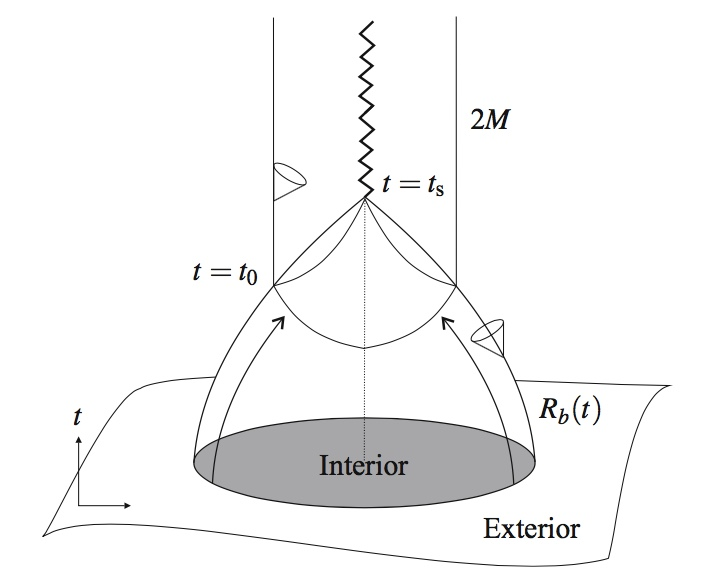
\includegraphics[scale=0.25] {figures/EFCollapse.jpeg}
      \end{figure}
	\end{center}	
\end{frame}

\begin{frame}{Gravitational Collapse of a Homogeneous Cloud of Dust}
\framesubtitle{Eddington-Finkelstein Diagram}
	\begin{center}
      \begin{figure}
      	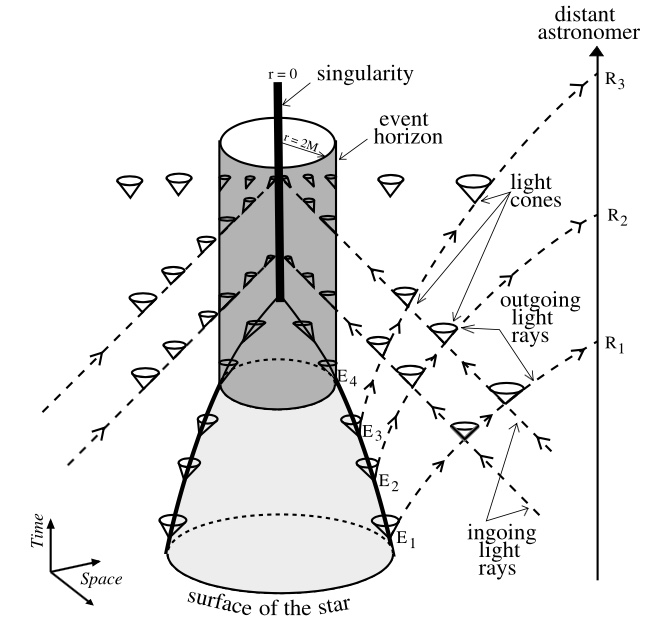
\includegraphics[scale=0.25] {figures/EFCollapse2.jpeg}
      \end{figure}
	\end{center}	
\end{frame}

\begin{darkframes}

\subsection{Inhomogeneous Dust Collapse}
\begin{frame}
	\huge
    Inhomogeneous Dust Collapse
\end{frame}

\begin{frame}{Inhomogeneous Dust Collapse}
    $\rho$ depends on both $t$ and $r$, and thus\\
    \bigskip
    \pause
    $\rho = \rho(t,r)$\\
    $m = m(r)$\\
    $b = b(r)$\\
    $a = a(t,r)$
\end{frame}

\begin{frame}{Inhomogeneous Dust Collapse}
    The simplest form for the function $m(r)$ is
    $$m(r) = m_0 + m_2 r^2$$
    \pause
    This function defines the density interms of the two parameter $m_0$ and $m_2$.\\
    \pause
    The condition that $\rho$ must be a decreasing function of $r$ implies that $m_2 <0$.\\
    \bigskip
    \pause
    \footnotesize
    * $m_1=0$ in order to have a non divergent density. 
\end{frame}

\begin{frame}{Inhomogeneous Dust Collapse}
    The equation
    $$ \dot{R}^2 = \frac{F}{R} + f$$
    gives this time
    $$r \dot{a(t,r)} = - \sqrt[]{\frac{mr^2}{ra} + b r^2}$$
    \pause
    $$\dot{a(t,r)} = - \sqrt[]{\frac{m}{a} + b}$$
\end{frame}

\begin{frame}{Inhomogeneous Dust Collapse}
    In the marginally bound case, $b=0$, it gives
    \pause
    $$\dot{a(t,r)} = - \sqrt[]{\frac{m(r)}{a}}$$
    \pause
    $$\sqrt[]{a(t,r)} da = - \sqrt[]{m(r)}dt$$
    \pause
 	$$\frac{2}{3} a^{3/2}(t,r) - \frac{2}{3} a^{3/2}(0,r) = -\sqrt[]{m(r)} t$$
\end{frame}

\begin{frame}{Inhomogeneous Dust Collapse}
    The value of the initial condition was supposed as $a(0)=1$. Thus
    $$a(t,r) = \left[ 1-\frac{3\sqrt[]{m(r)}}{2}t \right]^{2/3}$$
    \pause
    This equation shows how each shell of the distribution (each $r$) collapses with a different scale factor and with a different velocity.
\end{frame}

\begin{frame}{Inhomogeneous Dust Collapse}
	The time to reach the singularity and the horizon are, respectively,
    \pause
    $$t_s (r) = \frac{2}{3\sqrt[]{m(r)}}$$
    \pause
    $$t_H (r) = \frac{2}{3\sqrt[]{m(r)}} - \frac{2}{3} m(r) r^3$$
\end{frame}

\begin{frame}{Inhomogeneous Dust Collapse}
	Using $m(r) = m_0 + m_2 r^2$ gives the functions
	$$t_s (r) = \frac{2}{3\sqrt[]{m_0 + m_2 r^2}}$$
    $$t_H (r) = \frac{2}{3\sqrt[]{m_0 + m_2 r^2}} - \frac{2}{3} r^3 \left(m_0 + m_2 r^2 \right)$$
\end{frame}

\end{darkframes}

\begin{frame}{Gravitational Collapse of a Inhomogeneous Cloud of Dust}
\framesubtitle{Eddington-Finkelstein Diagram}
	\begin{center}
      \begin{figure}
      	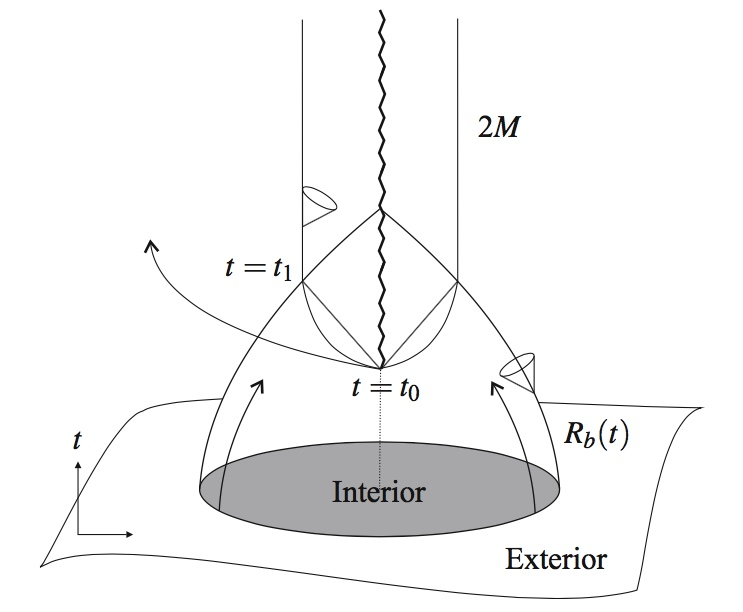
\includegraphics[scale=0.25] {figures/EFCollapseInhomogeneous.jpeg}
      \end{figure}
	\end{center}	
\end{frame}

\begin{darkframes}

  		\begin{frame}{Next Lecture}
        	\Large
			{06. Black Holes Astrophysics}
		\end{frame}
  
  \end{darkframes}
\end{document}
